\documentclass[residuals.tex]{subfiles}
\begin{document}
	
\section{Measures of Influence}
The impact of an observation on a regression fitting can be determined by the difference between the estimated regression coefficient of a model with all observations and the estimated coefficient when the particular observation is deleted. The measure DFBETA is the studentized value of this difference.

Influence arises at two stages of the LME model. Firstly when $V$ is estimated by $\hat{V}$, and subsequent
estimations of the fixed and random regression coefficients $\beta$ and $u$, given $\hat{V}$.

\subsection{Cook's Distance}
Cook's distance or Cook's D is a commonly used estimate of the influence of a data point when performing least squares regression analysis.

In a practical ordinary least squares analysis, Cook's distance can be used in several ways: to indicate data points that are particularly worth checking for validity; to indicate regions of the design space where it would be good to be able to obtain more data points. 

It is named after the American statistician R. Dennis Cook, who introduced the concept in 1977.

Cook's distance measures the effect of deleting a given observation. Data points with large residuals (outliers) and/or high leverage may distort the outcome and accuracy of a regression. Points with a large Cook's distance are considered to merit closer examination in the analysis.

\subsubsection{Computation}
\[ D_i = \frac{ \sum_{j=1}^n (\hat Y_j\ - \hat Y_{j(i)})^2 }{p \ \mathrm{MSE}} .\]
The following are the algebraically equivalent expressions (in case of simple linear regression):

\[ D_i = \frac{e_i^2}{p \ \mathrm{MSE}}\left[\frac{h_{ii}}{(1-h_{ii})^2}\right],\]
\[ D_i = \frac{ (\hat \beta - \hat {\beta}^{(-i)})^T(X^TX)(\hat \beta - \hat {\beta}^{(-i)}) } {(1+p)s^2}.\]
In the above equations:

\begin{itemize}
	\item $\hat Y_j \,$ is the prediction from the full regression model for observation j;
	\item $\hat Y_{j(i)}\,$ is the prediction for observation j from a refitted regression model in which observation i has been omitted;
	\item $h_{ii} \,$ is the i-th diagonal element of the hat matrix 
	\[ \mathbf{X}\left(\mathbf{X}^T\mathbf{X}\right)^{-1}\mathbf{X}^T;\]
	\item $e_i \,$ is the crude residual (i.e., the difference between the observed value and the value fitted by the proposed model);
	\item $\mathrm{MSE} \,$ is the mean square error of the regression model;
	\item $p$ is the number of fitted parameters in the model
\end{itemize}

\subsubsection{DFBETA}

The DFBETA statistic for measuring the influence of 
the th observation is defined as the one-step approximation to 
the difference in the MLE of the regression parameter vector and 
the MLE of the regression parameter vector without the th 
observation. This one-step approximation assumes a Fisher 
scoring step, and is given by

%EQUATION


\subsubsection{DFFITS} %1.16.1
DFFITS is a statistical measured designed to a show how influential an observation is in a statistical model. It is closely related to the studentized residual.
\begin{displaymath} DFFITS = {\widehat{y_i} -
	\widehat{y_{i(k)}} \over s_{(k)} \sqrt{h_{ii}}} \end{displaymath}


\subsubsection{PRESS} %1.16.2
The prediction residual sum of squares (PRESS) is an value associated with this calculation. When fitting linear models, PRESS can be used as a criterion for model selection, with smaller values indicating better model fits.
\begin{equation}
PRESS = \sum(y-y^{(k)})^2
\end{equation}


\begin{itemize}
	\item $e_{-Q} = y_{Q} - x_{Q}\hat{\beta}^{-Q}$
	\item $PRESS_{(U)} = y_{i} - x\hat{\beta}_{(U)}$
\end{itemize}

\subsubsection{DFBETA} %1.16.3
\begin{eqnarray}
DFBETA_{a} &=& \hat{\beta} - \hat{\beta}_{(a)} \\
&=& B(Y-Y_{\bar{a}}
\end{eqnarray}
%-------------------------------------------------------------- %
\newpage

\subsection{Influential Observations : DFBeta and DFBetas}
% http://stats.stackexchange.com/questions/22161/how-to-read-cooks-distance-plots
Cook's distance refers to how far, on average, predicted y-values will move if the observation in question is dropped from the data set. dfbeta refers to how much a parameter estimate changes if the observation in question is dropped from the data set. Note that with k covariates, there will be k+1 dfbetas (the intercept,$\beta_0$, and 1 $\beta$ for each covariate). Cook's distance is presumably more important to you if you are doing predictive modeling, whereas dfbeta is more important in explanatory modeling.


\subsection{Leverage}
leverage is a term used in connection with regression analysis and, in particular, in analyses aimed at identifying those observations that are far away from corresponding average predictor values. Leverage points do not necessarily have a large effect on the outcome of fitting regression models.

Leverage points are those observations, if any, made at extreme or outlying values of the independent variables such that the lack of neighboring observations means that the fitted regression model will pass close to that particular observation.[1]

Modern computer packages for statistical analysis include, as part of their facilities for regression analysis, various quantitative measures for identifying influential observations: among these measures is partial leverage, a measure of how a variable contributes to the leverage of a datum.

%-------------------------------------------------------------------------------------------%
\newpage
	
\section{Influential Points in Regression}
% - http://stattrek.com/regression/influential-points.aspx
 

%ometimes in regression analysis, a few data points have disproportionate effects on the slope of the regression equation. In this lesson, we describe how to identify those influential points.


\begin{figure}
\centering
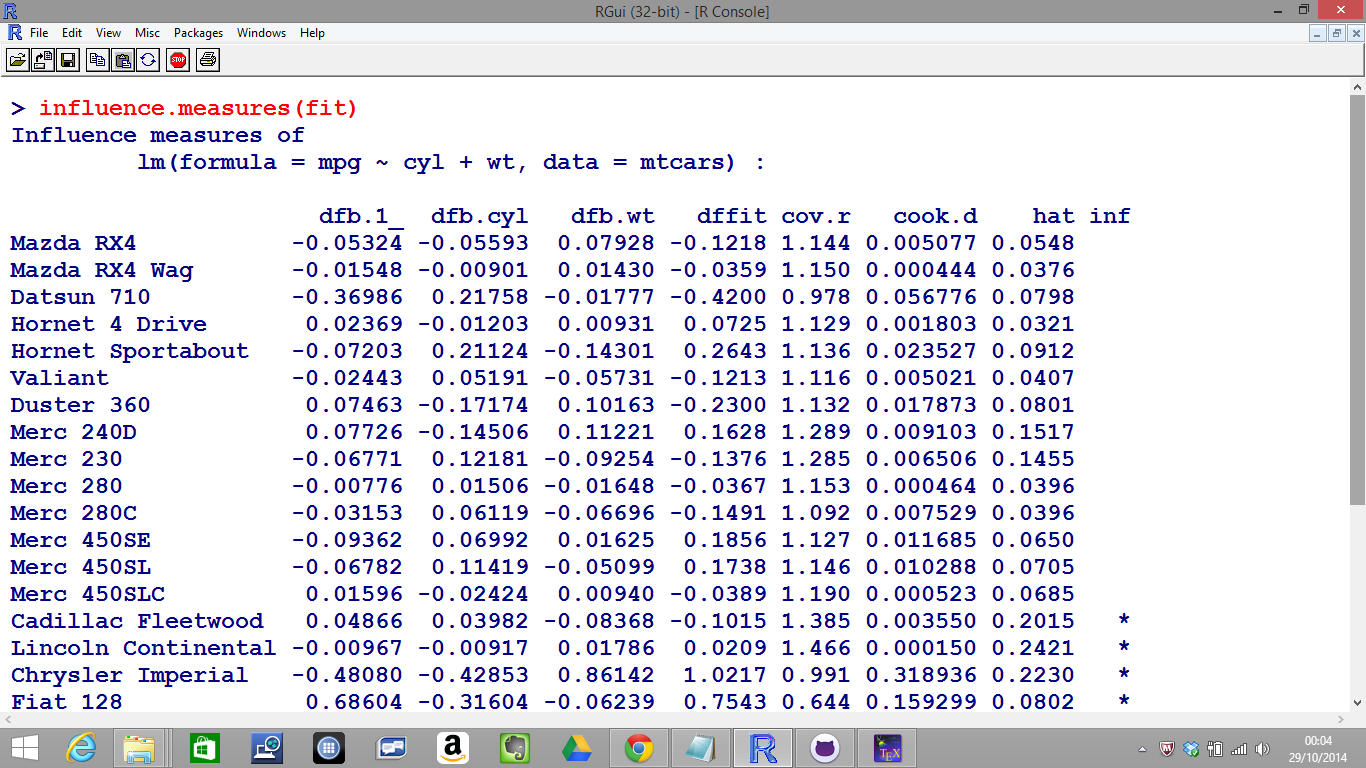
\includegraphics[width=1.1\linewidth]{Screenshot2}
\caption{}
\label{fig:Screenshot2}
\end{figure}


\begin{verbatim}
inflm.fit <- influence.measures(fit)
which(apply(inflm.fit$is.inf, 1, any))
\end{verbatim}
%-------------------------------------------------------------------------------------------%
\newpage
\section{Leverage and Influence}
\subsection{Influence}
The influence of an observation can be thought of in terms of how much the predicted scores for other observations would differ if the observation in question were not included. 

Cook's D is a good measure of the influence of an observation and is proportional to the sum of the squared differences between predictions made with all observations in the analysis and predictions made leaving out the observation in question. If the predictions are the same with or without the observation in question, then the observation has no influence on the regression model. If the predictions differ greatly when the observation is not included in the analysis, then the observation is influential.


\subsection{Leverage}
% http://onlinestatbook.com/2/regression/influential.html
% Leverage
The leverage of an observation is based on how much the observation's value on the predictor variable differs from the mean of the predictor variable. The greater an observation's leverage, the more potential it has to be an influential observation. 

For example, an observation with a value equal to the mean on the predictor variable has no influence on the slope of the regression line regardless of its value on the criterion variable. On the other hand, an observation that is extreme on the predictor variable has the potential to affect the slope greatly.

\subsubsection{Calculation of Leverage (h)}
The first step is to standardize the predictor variable so that it has a mean of 0 and a standard deviation of 1. Then, the leverage (h) is computed by squaring the observation's value on the standardized predictor variable, adding 1, and dividing by the number of observations.

% Extreme X value
% Extreme Y value
% Extreme X and Y 
% Distant data point

\subsection{Influential Points}

An influential point is an outlier that greatly affects the slope of the regression line. One way to test the influence of an outlier is to compute the regression equation with and without the outlier.

This type of analysis is illustrated below. The scatter plots are identical, except that the plot on the right includes an outlier. The slope is flatter when the outlier is present (-3.32 vs. -4.10), so this outlier would be considered an influential point.

\subsection{Without Outlier}

% With Outlier

\begin{itemize}
\item Regression equation: $\hat{y} = 104.78 - 4.10x$
\item Coefficient of determination: $R^2 = 0.94$ 
\end{itemize}
\begin{itemize}
\item Regression equation: $\hat{y} = 97.51 - 3.32x$
\item Coefficient of determination: $R^2 = 0.55$ 
\end{itemize}

The charts below compare regression statistics for another data set with and without an outlier. Here, the chart on the right has a single outlier, located at the high end of the X axis (where x = 24). As a result of that single outlier, the slope of the regression line changes greatly, from -2.5 to -1.6; so the outlier would be considered an influential point.

% Without Outlier
% With Outlier

% Regression equation: ŷ = 92.54 - 2.5x
% Slope: b0 = -2.5
% Coefficient of determination: R2 = 0.46 

% Regression equation: ŷ = 87.59 - 1.6x
% Slope: b0 = -1.6
% Coefficient of determination: R2 = 0.52 


Sometimes, an influential point will cause the coefficient of determination to be bigger; sometimes, smaller. In the first example above, the coefficient of determination is smaller when the influential point is present (0.94 vs. 0.55). In the second example, it is bigger (0.46 vs. 0.52).

If your data set includes an influential point, here are some things to consider.

%--------------------------------------------------------------------------------------%

\begin{itemize}
\item An influential point may represent bad data, possibly the result of measurement error. If possible, check the validity of the data point.

\item Compare the decisions that would be made based on regression equations defined with and without the influential point. If the equations lead to contrary decisions, use caution.

\end{itemize}
%Test Your Understanding of This Lesson
%
%In the context of regression analysis, which of the following statements are true?
%
% I. When the data set includes an influential point, the data set is nonlinear. 
%II. Influential points always reduce the coefficient of determination. 
%III. All outliers are influential data points. 
%
%(A) I only 
%(B) II only 
%(C) III only 
%(D) All of the above 
%(E) None of the above 
%
%Solution
%
%The correct answer is (E). Data sets with influential points can be linear or nonlinear. In this lesson, we went over an example in which an influential point increased the coefficient of determination. With respect to regression, outliers are influential only if they have a big effect on the regression equation. Sometimes, outliers do not have big effects. For example, when the data set is very large, a single outlier may not have a big effect on the regression equation.

\subsection{Summary of Influence Statistics}
\begin{itemize}
	\item	\textbf{Studentized Residuals} – Residuals divided by their estimated standard errors (like t-statistics). Observations with values larger than 3 in absolute value are considered outliers.
	\item	\textbf{Leverage Values (Hat Diag)} – Measure of how far an observation is from the others in terms of the levels of the independent variables (not the dependent variable). Observations with values larger than $2(k+1)/n$ are considered to be potentially highly influential, where k is the number of predictors and n is the sample size.
	\item	\textbf{DFFITS} – Measure of how much an observation has effected its fitted value from the regression model. Values larger than $2\sqrt{(k+1)/n}$ in absolute value are considered highly influential. %Use standardized DFFITS in SPSS.
	\item	\textbf{DFBETAS} – Measure of how much an observation has effected the estimate of a regression coefficient (there is one DFBETA for each regression coefficient, including the intercept). Values larger than 2/sqrt(n) in absolute value are considered highly influential.
	\\
	The measure that measures how much impact each observation has on a particular predictor is DFBETAs The DFBETA for a predictor and for a particular observation is the difference between the regression coefficient calculated for all of the data and the regression coefficient calculated with the observation deleted, scaled by the standard error calculated with the observation deleted. 
	
	\item	\textbf{Cook’s D} – Measure of aggregate impact of each observation on the group of regression coefficients, as well as the group of fitted values. Values larger than 4/n are considered highly influential.
\end{itemize}


\end{document}